\chapter{緒言}
\thispagestyle{myheadings}

\section{背景}
認知症とは,記憶,判断などの認知機能が後天的な脳の障害によって持続性に低下し,日常生活や社会生活に支障をきたすようになる状態である [1].認知症は加齢とともに増加するため,高齢者数の増大とともに,認知症の有病者数は増大する[2].平成29年度の内閣府による65歳以上の認知症高齢者数と将来推計[3]では,図1.1に示すように平成24年は認知症高齢者数426万人,平成37年には推計で約700万人になると報告されており,認知症の発症および進行を遅らせる予防の重要性が増している[4].認知症の予防を目的とした非薬物療法として運動,社会参加,対人交流,知的活動の実施などが挙げられる[5].この中でも運動は,地方自治体が高齢者向けの運動教室を広く展開しており,介護予防事業の中核を果たしている[4][6].

 運動教室で実施されている運動プログラムの一つにコグニサイズ(cognicise)がある[7].コグニサイズは,国立長寿医療研究センター[8]が開発した運動と計算やしりとりなどの認知課題を同時に負荷する認知症予防トレーニングである.運動教室でのコグニサイズの実施の様子を図1.2に示す.運動の種類によってコグニステップ,コグニラダー,コグニウォークなど呼称が異なる[9].コグニステップの実施方法を図1.3に示す.文献[7]では,認知症予防の効果があるコグニサイズの条件として,1)運動は全身を使った中強度程度の負荷がかかるものであり、脈拍数が上昇する,2)運動と同時に実施する認知課題によって、運動の方法や認知課題自体をたまに間違えてしまう程度の負荷がかかっているとしている.また,個人の身体状況に応じて,運動と認知課題の負荷を調整することが重要だとしている.しかし,運動教室で実施される集団でのコグニサイズは,参加者全員に対する負荷が一定のため,認知症予防の効果が得られない参加者が現れる可能性がある[10].

 そこで本研究では,ICTを使用し,運動教室で実施される集団でのコグニサイズにおいて、個別に認知課題の負荷を調整する助けを行う.認知課題の正誤判定を自動で行い,正誤判定の集計結果を正答率として蓄積していくことで,過去の認知課題の正答率に応じて,個別に認知課題の負荷を調整可能なシステムを開発する.運動教室の参加者が提案システムを使用することによって,個別に認知症予防の効果があるコグニサイズを実施できることが期待される.

\begin{comment}
リハビリテーション(以下リハビリ)とは,障害の原因となる機能の回復を図る訓練である.下肢リハビリの風景を図\ref{fig:rihabiri}に示す.リハビリは,主に理学療法士が計画を立案・施行し,患者の機能回復や障害の改善を目標としている.社会の高齢化が進み,リハビリを必要とする患者の数が増加しているが理学療法士の人手不足の問題を抱えている\cite{理学療法士}.そのため,機械やロボット技術を使用したリハビリ装置の導入に向けて研究が進められている\cite{フィットネスマシン}.機械を使用したリハビリ装置の1つである,下肢リハビリ装置を図\ref{fig:smart-1}--\ref{fig:smart-2}に示す.下肢リハビリ装置は,下肢リハビリの動作と連動した,ゲームをしながら楽しむリハビリ装置である.その他に,健常者の怪我予防や筋力トレーニングにも使用されている.また,機械を使用したリハビリ装置において,寝たきりの患者が利用可能なベット型の下肢リハビリ装置が開発されている.ベット型の下肢リハビリ装置を図\ref{fig:tadouhokou}に示す.ベッド型の下肢リハビリ装置は,患者が仰向けの体勢になり,装置の下肢部分が上下に動作することで歩行動作の機能回復を図る.下肢リハビリを患者が行う際,歩行動作改善のため,正常な歩行を想像することが重要であると報告されている\cite{歩行イメージ再学習}.現状のベッド型の下肢リハビリ装置のみでは患者が天井を見上げ,正常な歩行を想像することが難しく,また,退屈であるという問題点も挙げられる.

そこで本研究では,HMD (Head Mounted Display)を使用し,患者が天井を見上げる退屈さを解消し,正常な歩行の想像の助けを行う.ベッド型の下肢リハビリ装置の動きと仮想空間内に配置したキャラクタの視界移動を同期させることで,歩行を行う視覚の感覚を提示可能なシステムを開発する.HMDを図\ref{fig:Oculus}に示す.患者が提案システムを使用することによって,正常な歩行の想像の一助となることが期待される.また,歩行を疑似体験することで患者が「早く治したいという気持ち」にするモチベーションの維持も期待される.
\end{comment}

\begin{figure}[tbp]
	\centering
			\includegraphics[width=0.9\textwidth]{chap1-figure/rihabiri.eps}
	\caption{下肢リハビリ風景}
	\label{fig:rihabiri}
\end{figure}

\begin{figure}[tbp]
	\centering
			\includegraphics[width=0.9\textwidth]{chap1-figure/s-1.eps}
	\caption{下肢リハビリ器具正面図(文献\cite{フィットネスマシン}より引用)}
	\label{fig:smart-1}
\end{figure}

\begin{figure}[tbp]
	\centering
			\includegraphics[width=0.9\textwidth]{chap1-figure/s-2.eps}
	\caption{下肢リハビリ器具側面図(文献\cite{フィットネスマシン}より引用)}
	\label{fig:smart-2}
\end{figure}

\begin{figure}[tbp]
	\centering
			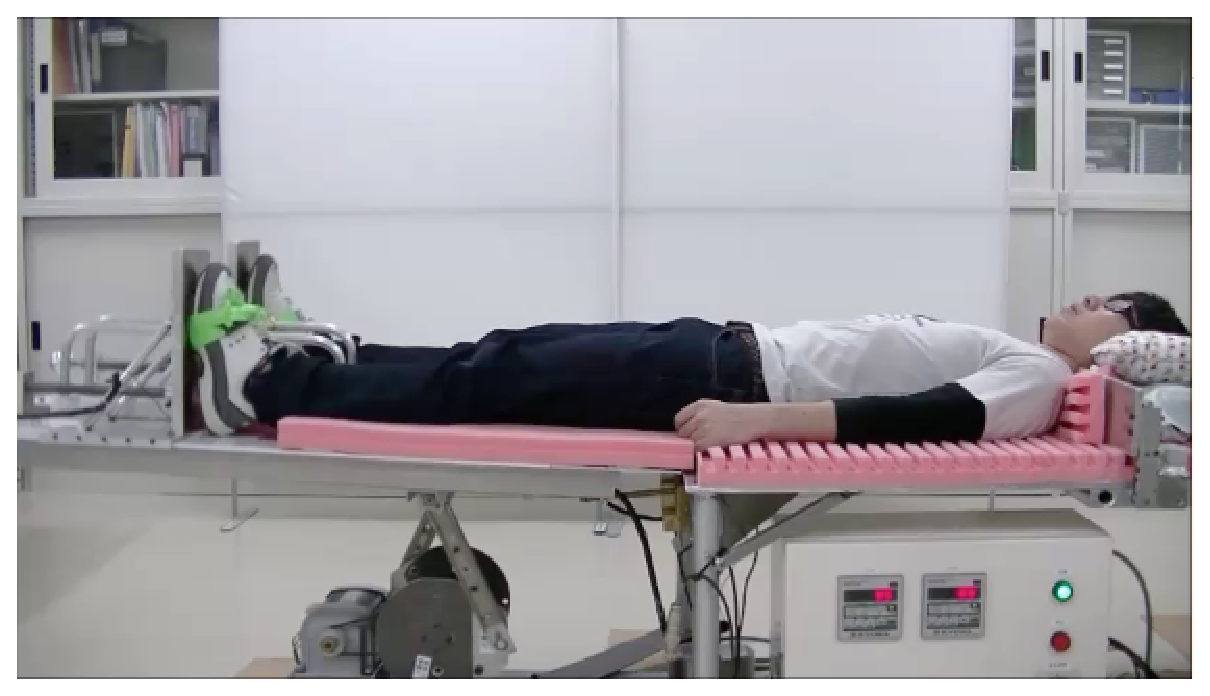
\includegraphics[width=0.9\textwidth]{chap1-figure/tadouhoku.eps}
	\caption{ベット型下肢リハビリ器具}
	\label{fig:tadouhokou}
\end{figure}

\begin{figure}[tbp]
	\centering
			\includegraphics[width=0.7\textwidth]{chap1-figure/Oculus.eps}
	\caption{HMD}
	\label{fig:Oculus}
\end{figure}

\section{関連研究}
本節では,機械を使用した下肢リハビリに関する研究と歩行感覚提示装置に使用するディスプレイに関する印象調査に関連する研究について述べる.維持期脳卒中患者に対して歩行感覚提示装置を用いた歩行トレーニングを行い,その効果の持続性の検討\cite{筑波歩行感覚提示}が田中らによって行われている.棚からの歩行感覚提示装置を図\ref{fig:tukuba}に示す.歩行感覚提示装置は,通常の歩行に近い動作かつ,通常の歩行と同じ1m/sの歩行速度を実現可能な装置である.患者は球面型ディスプレイ内を歩く構造となっている.入院前の健康状態の歩幅で自宅付近を歩く疑似体験をすることで,患者自身が早く治したいという気持ちになり,リハビリに対するモチベーションが向上するという精神面での効果も報告されている.しかし,寝たきりの患者は対象とされていない問題点がある.

\begin{figure}[tbp]
	\centering
			\includegraphics[width=0.5\textwidth]{chap1-figure/tukuba.eps}
	\caption{没入型歩行感覚提示装置全景(文献\cite{筑波歩行感覚提示画像}より引用)}
	\label{fig:tukuba}
\end{figure}

高齢者の自立・社会参加の前提となる歩行機能および歩行訓練に着目し,バーチャルリアリティ(VR: Virtual Reality)を活用した歩行訓練器具\cite{日立}が藤江らによって開発されている.藤江らによる歩行訓練機器を図\ref{fig:hitachi}に示す.リハビリ患者の歩行機能の改善を目指し,自立歩行によって実写映像が切り替わるシステムとなっている.VRを活用しリハビリ患者の訓練意欲を高める試みがされている.リハビリ患者に対して,立体視可能な映像を流した結果,映像に集中していたという結果が報告されている.そのことから,HMDを使用することがリハビリへの集中に繋がることも期待される.
\begin{figure}[tbp]
	\centering
			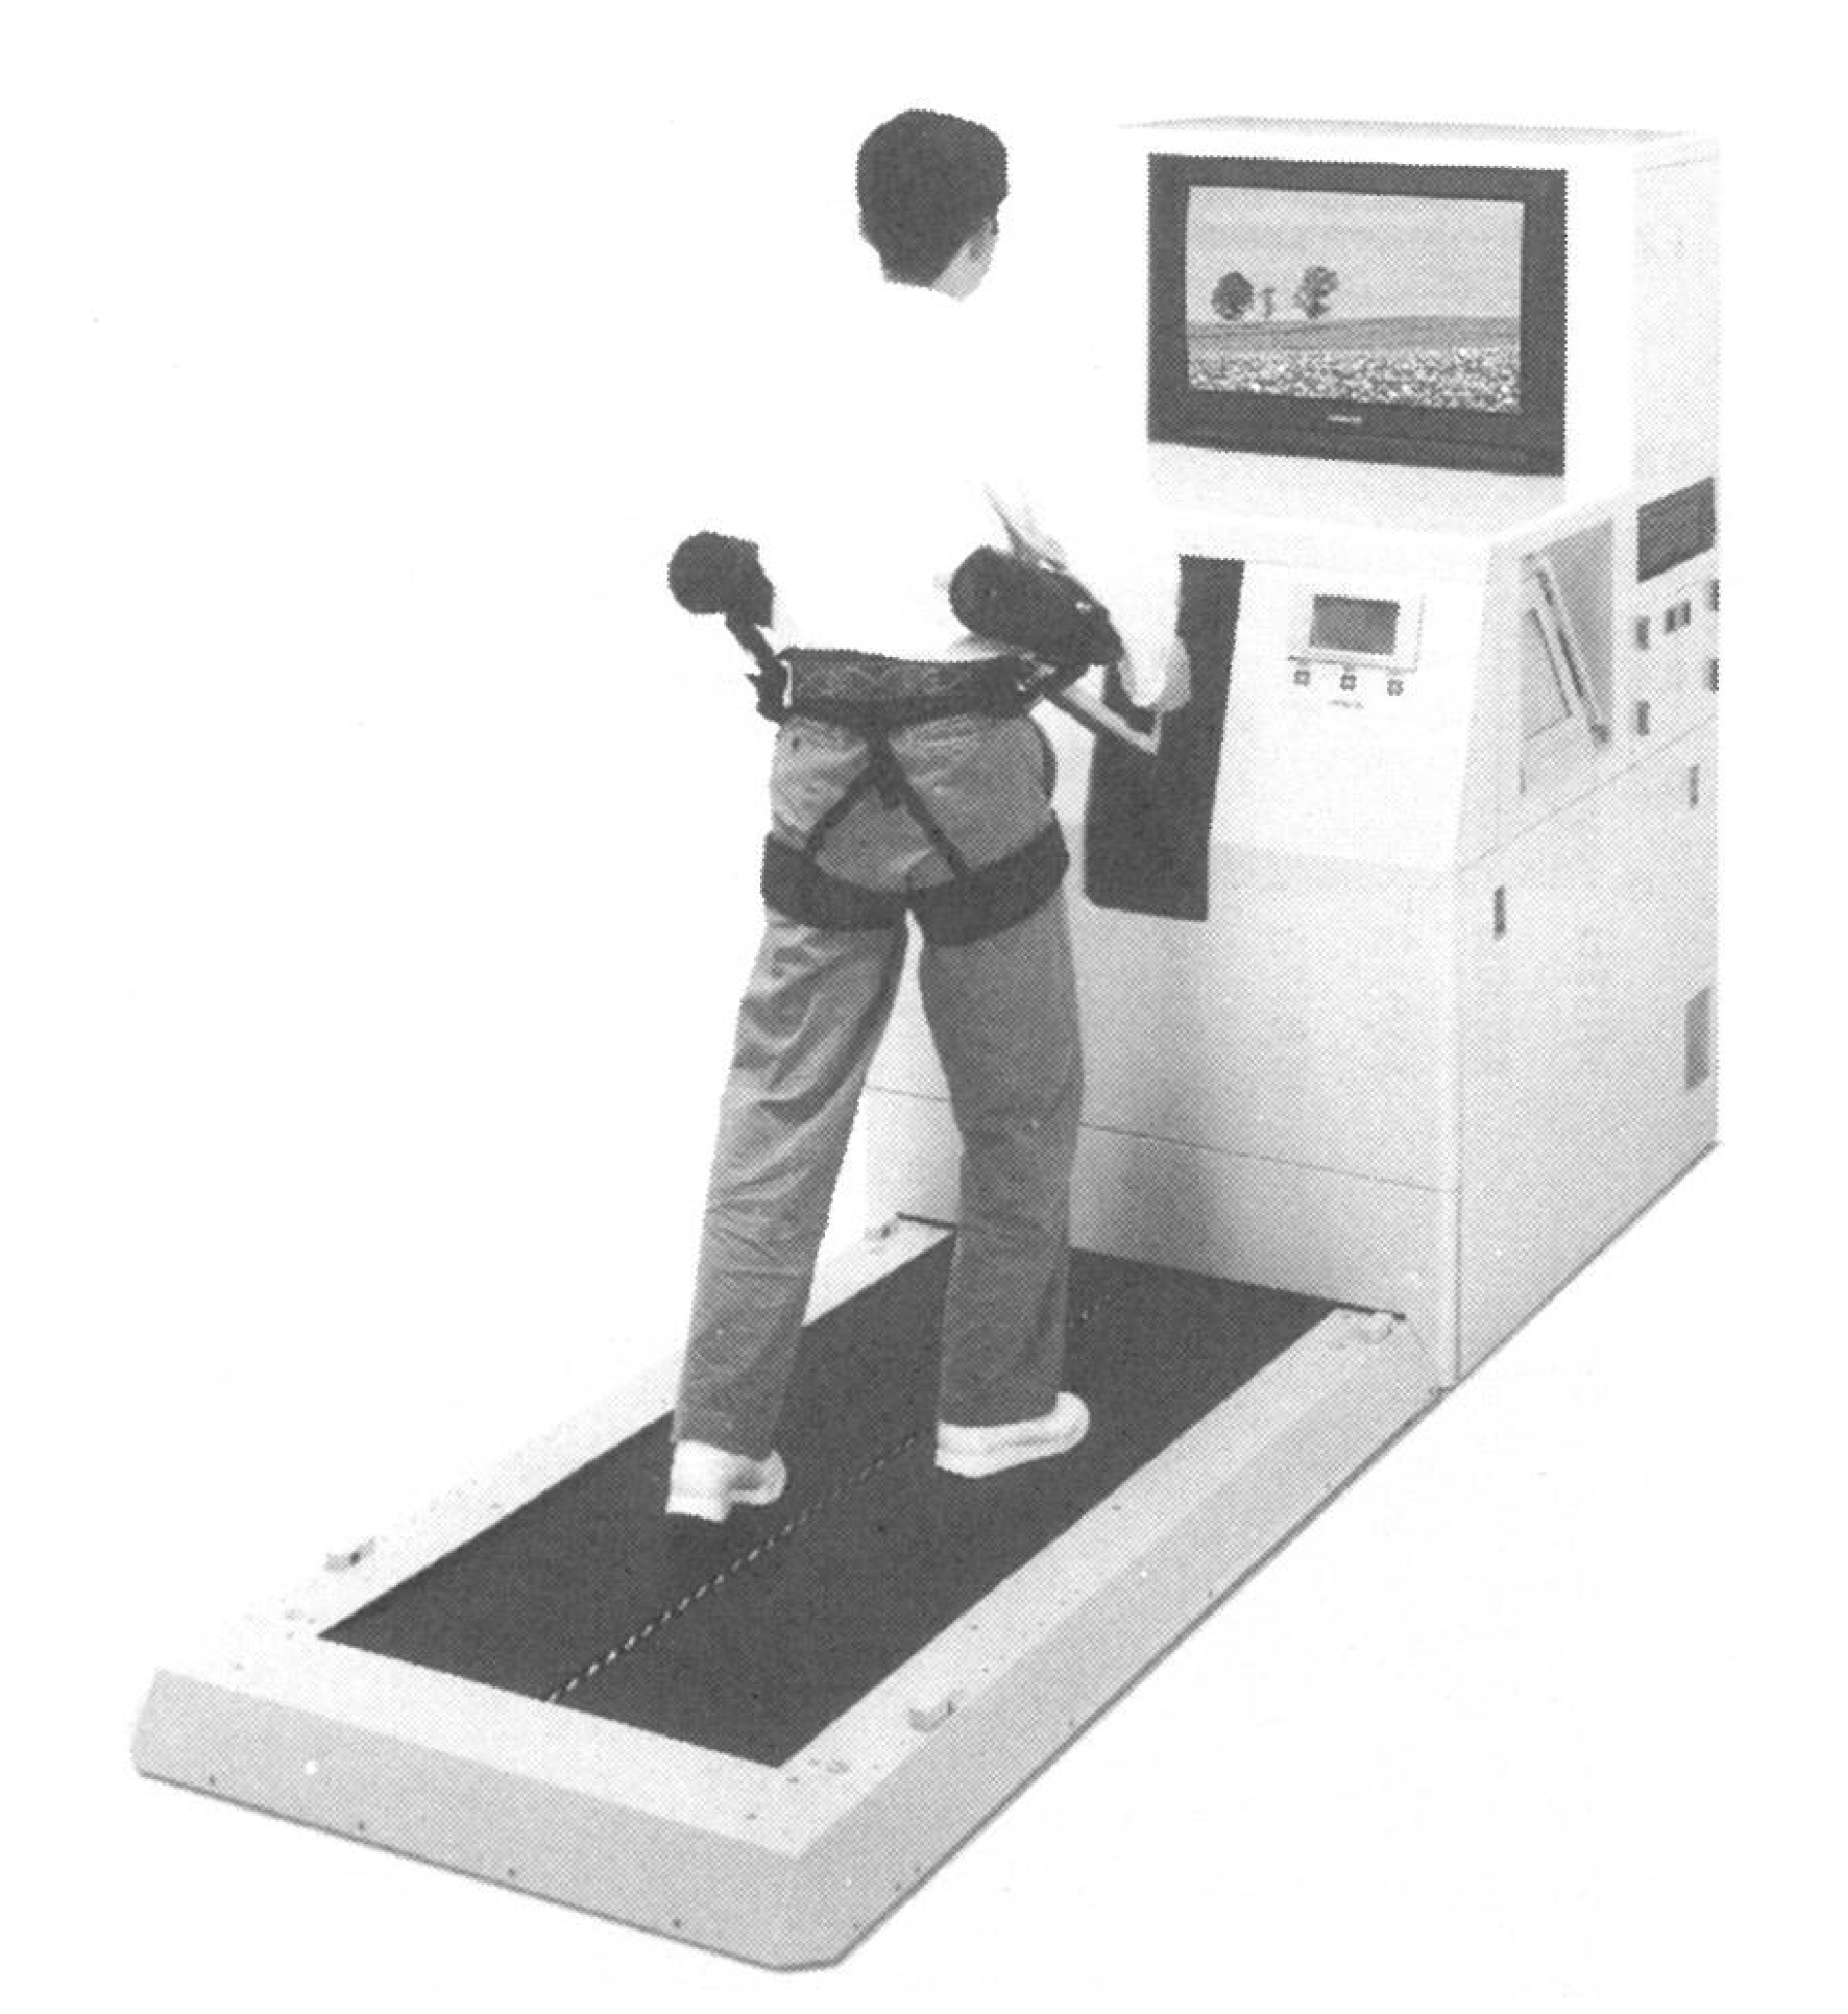
\includegraphics[width=0.5\textwidth]{chap1-figure/VRhokou.eps}
	\caption{バーチャルリアリティを活用した歩行訓練機器(文献\cite{日立}より引用)}
	\label{fig:hitachi}
\end{figure}

歩行感覚提示に使用するディスプレイの印象評価\cite{ディスプレイの違い}が小林らによって報告されている.ロコモーション・インターフェース\cite{ロコモーション}(LI: Locomotion Interface)を提示するディスプレイとして,プラズマディスプレイとHMDとスクリーンの3タイプのディスプレイを用い,ユーザに与える感覚を測定し分析が行われている.ロコモーション・インターフェースとは,VRにおいて,あたかも現実で歩いているような感覚を体感できる装置である.小林らの調査の結果,ディスプレイの違いによってユーザの感覚に差は僅差であったと報告されている.そのことから,ベッド型の下肢リハビリ装置には,着脱可能なHMDの利用が容易であると考えられる.

いずれの関連研究も自立で立ち上がることが可能なリハビリ患者を対象としており,寝たきりの患者は対象とされていない.
そこで本研究では,寝たきりの患者も対象とし,下肢リハビリを行う際の退屈さや歩行の想像の助けを行うシステムの開発をする.

\section{本研究の目的}
本研究目的は,HMDを使用し,患者が天井を見上げる退屈さを解消し,正常な歩行の想像の助けを行う.ベッド型の下肢リハビリ装置の動きと仮想空間内に配置したキャラクタの視界移動を同期させることで,歩行を行う視覚の感覚を提示可能なシステムを開発する.患者が提案システムを使用することによって,正常な歩行の想像の一助となることが期待される.また,歩行を疑似体験することで患者が「早く治したいという気持ち」にするモチベーションの維持も期待される.
\section{論文の構成}

本稿の構成について述べる.第2章では提案システムの概要と処理の流れについて述べ,第3章では,提案システムに関するSD法を使用したアンケートと記述式のアンケートで印象の評価を行う.そして,評価の結果からの考察を述べる.第4章では,以上で述べたことをまとめ,実験の考察の課題に基づき今後の課題を明らかにする.

% Local Variables: 
% mode: japanese-LaTeX
% TeX-master: "root"
% End: 
